\documentclass[a4paper]{article}
\usepackage[margin=1.25in]{geometry}
\setcounter{tocdepth}{2}

% text
\usepackage{mathptmx}
\usepackage{textcomp}
\usepackage{lipsum}
\linespread{1.2}

% header and footer
\usepackage{fancyhdr}
\pagestyle{fancy}
\newcommand{\pageauthor}{}
\lhead{\pageauthor}
\rhead{\thepage}

% links
\usepackage{bookmark}
\usepackage{hyperref}
\usepackage[numbib]{tocbibind}

% figures
\usepackage{float}
\usepackage{graphicx}
\usepackage{caption}
\usepackage{subcaption}

% tables
\usepackage{tabularx}
\usepackage{multirow}
\newcolumntype{L}{>{\centering\arraybackslash}X}

% maths
\usepackage{amsmath}
\usepackage{amssymb}
\usepackage{mathtools}
\allowdisplaybreaks
\newcommand{\raisedtilde}{\raisebox{0.5ex}{\texttildelow}}
\DeclarePairedDelimiter\bra{\langle}{\rvert}
\DeclarePairedDelimiter\ket{\lvert}{\rangle}
\DeclarePairedDelimiterX\braket[2]{\langle}{\rangle}{#1\,\delimsize\vert\,\mathopen{}#2}

% theorem
\usepackage{xpatch}
\usepackage{amsthm}
\newtheorem{theorem}{Theorem}
\newtheorem{definition}{Definition}[section]
\xpretocmd{\proof}{\setlength{\parindent}{0pt}}{}{}

% meta
\title{Quantum Channels: Transition from Classical to Quantum Channels}
\author{Himanshu Singh \and Raagav Ramakrishnan \and Shreyas Sinha \and Yash Seri}
\date{November 21, 2024}

\begin{document}

% front
\maketitle
\tableofcontents

\renewcommand{\pageauthor}{Shreyas Sinha}
\section{Introduction}

\begin{frame}{Introduction}
    In this presentation, we will be discussing quantum channels and how they developed from classical channels. But before that, we need to define what quantum channels
    are and what they operate on.
    Quantum channels operate on Density Matrices, which are mathematical constructs that hold all information about a quantum state. They can be defined as:
    \begin{equation}
        \rho = \sum_{i}p_i | \psi_i \rangle \langle \psi_i |   
    \end{equation}
    where $\psi_i$ is the $i^th$ state occuring with probability $p_i$
\end{frame}

\begin{frame}{Introduction}
    A quantum channel acts as a linear \textit{Completely Positive Trace Preserving (CPTP)} map from one density matrix to the other. This means that the product state
    of the system and the environment stays positive throughout the transformation, and the trace remains constant. These two properties are essential for a channel to
    be physically viable and make sense in the real world.\\
    It is usually denoted with $\mathcal{N}$ and the state generated after the application of the channel is $\mathcal{N} (\rho)$.\\
    Generally, this channel is second one of the three steps that happen in the process of sending information from A to B, the others being encoding and decoding.
    These three steps have been illustrated in the following figures.
\end{frame}

\begin{frame}
    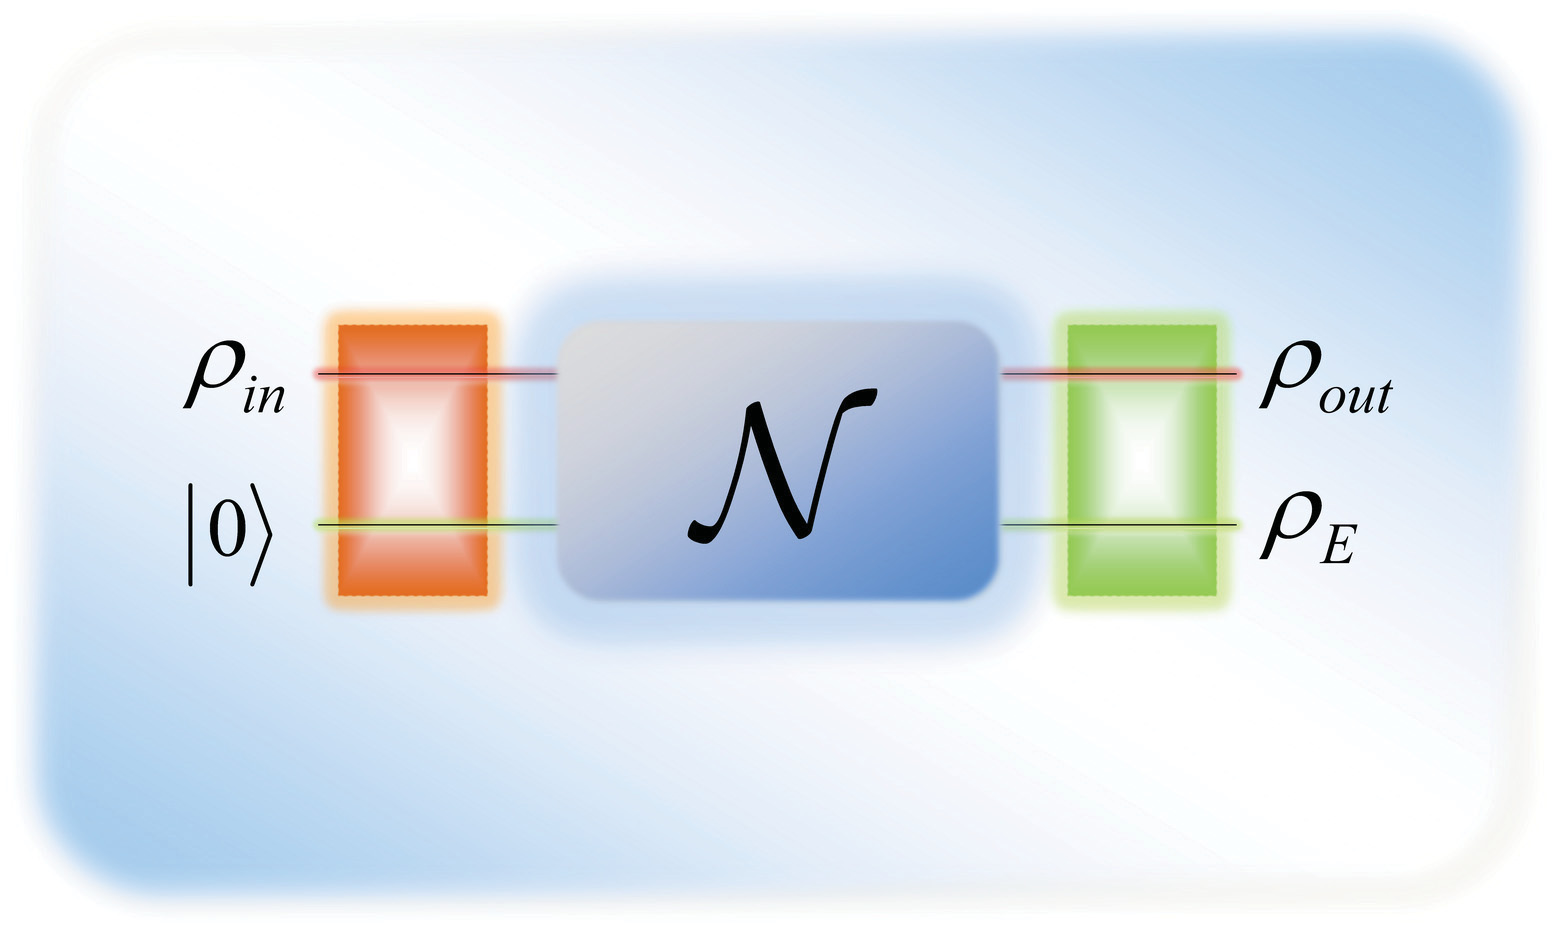
\includegraphics[scale=0.1]{channel2.png}
    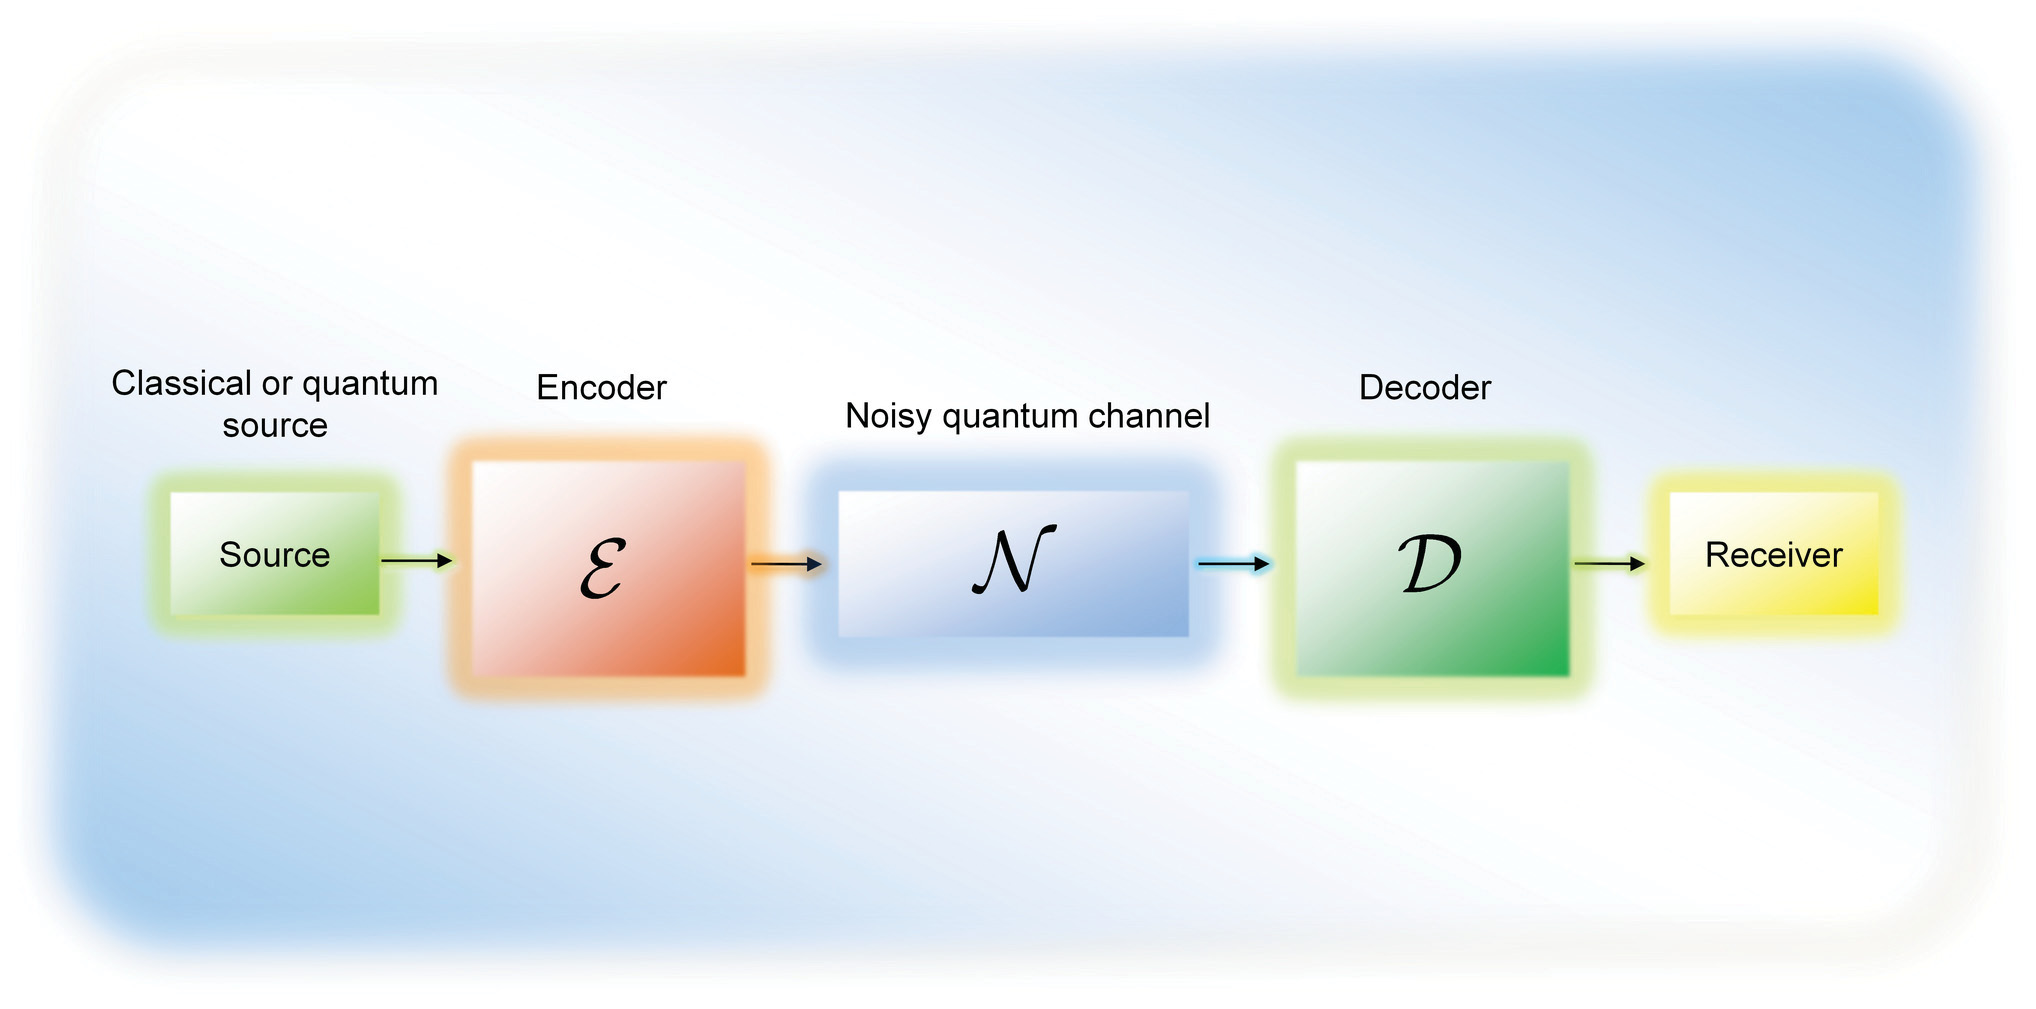
\includegraphics[scale=0.15]{channel1.png}
\end{frame}

\begin{frame}{Kraus Representation}
    Quantum channels are often represented in what is called the Kraus form (or the Choi-Kraus representation). In this form, quantum channels can be defined
    as linear combination in the following way:
    \begin{equation}
        \mathcal{N}(\rho) = \sum_i K_i \rho K_i^\dagger 
    \end{equation}
    where $\sum_i K_i^\dagger K_i = \mathbb{I} $\\
    The Kraus representation is very useful in as a tool for analysing quantum channels, and makes several problens easier to solve. Kraus operators and their
    uses show up at many useful places throughout Quantum information theory. It makes channels easier to understand as well, by decomposing them into several
    "sub-channels".
\end{frame}

\begin{frame}{Von Neumann Entropy}
    
\end{frame}

\begin{frame}{Quantum Relative Entropy}
    
\end{frame}

\begin{frame}{Quantum Mutual Information}
    
\end{frame}

\renewcommand{\pageauthor}{Yash Seri}
\section{Entropy and related quantities}

\subsection{Von Neumann Entropy}

\subsection{Conditional Entropy}

\subsection{Mutual Information}

\subsection{Relative Entropy}
\section{Accessible Information}
The Quantum no-cloning theorem establishes that quantum states cannot be perfectly cloned. This implies that there is an upper bound to the information that can be extracted from a quantum channel. The upper bound of information that is extractable from a quantum system is called the Holevo bound.\\
In classical systems, information is encoded deterministically, such as binary bits. In principle, all the encoded information can be accessed without limitations. In Quantum systems, however, information is encoded in quantum states, which can be superpositions or mixed states. This limits the amount of information that can be extracted from the system.
\newline
Let a sender(Alice) encode a classical variable X into a quantum state $\rho_x$. The receiver(Bob) attempts to decode X by measuring the quantum state. The accessible information is defined as the maximum classical mutual information between X and the output decoded Y:
\[
I_{accessible} = \text{max } I(X;Y)
\]
Where the maximum is taken over all possible measurements that can  be performed, represented by POVMs


\section{Holevo Bound}

\begin{frame}{Holevo Bound}
The Holevo bound is the upper bound of information that can be extracted from a quantum system, characterized by:
\[
\chi = I(\rho) - \sum_i p_i I(\rho_i).
\]
\end{frame}

\begin{frame}{Derivation of the Holevo Bound}
To prove this, consider a quantum system that encodes classical information represented by a distribution with probability \( p_x \) for each input \( x \), allowing us to define the classical state \( \rho_x \) as:
\[
\rho_X := \sum_x p_x |x\rangle \langle x|,
\]
where \( |x\rangle \) (ket x) represents a quantum state and \( \langle x| \) (bra x) represents the Hermitian conjugate of \( |x\rangle \).

Since each input is mapped to a quantum state \( \rho_x \), the combined state can be written as:
\[
\rho_{XQ} := \sum_x p_x |x\rangle \langle x| \otimes \rho_x.
\]
The received combined state is represented as:
\[
\rho := \text{tr}_X(\rho_{XQ}) = \sum_x p_x \rho_x,
\]
where \( \text{tr}_X \) represents the trace over \( \rho_{XQ} \).
\end{frame}

\begin{frame}{Derivation of the Holevo Bound}
To bound the maximum obtainable information, we need to bound the mutual information \( I(X : Y) \) with \( I(X : Q) \). From the monotonicity of quantum mutual information, we have:
\[
I(X : Q') \leq I(X : Q),
\]
and similarly:
\[
I(X : Y) \leq I(X : Q'Y).
\]

Combining these inequalities, we get:
\[
I(X : Y) \leq I(X : Q).
\]

Now, we simplify \( I(X : Q) \) as follows:
\begin{align*}
I(X : Q) &= I(X) + I(Q) - I(XQ) \\
         &= I(X) + I(\rho) + \text{tr}(\rho_{XQ} \log \rho_{XQ}) \\
         &= I(\rho) + \sum_x p_x \, \text{tr}(\rho_x \log \rho_x) \\
         &= I(\rho) - \sum_x p_x I(\rho_x),
\end{align*}
which gives the Holevo bound.
\end{frame}


\renewcommand{\pageauthor}{Raagav Ramakrishnan}
\section{Schumacher's Quantum Noiseless Channel Coding Theorem}

\lipsum

\section{Classical Capacity of a Quantum Channel}

\begin{frame}{Definition of Classical Capacity}
The classical capacity of a quantum channel \( \mathcal{N} \) is the maximum amount of classical information that can be transmitted per use of the channel with arbitrarily low error, as the number of channel uses goes to infinity. It is denoted by \( C(\mathcal{N}) \) and measured in bits per channel use.
\end{frame}

\begin{frame}{Types of Quantum Channels}
Quantum channels may be \textbf{noisy}, meaning they can alter or degrade the transmitted quantum states. Noise can arise from decoherence, loss, or other environmental factors. Common examples include depolarizing channels, dephasing channels, and amplitude damping channels.
\end{frame}

\begin{frame}{Formula for Classical Capacity}
The classical capacity \( C(\mathcal{N}) \) of a quantum channel \( \mathcal{N} \) is given by the regularized Holevo capacity:
\begin{equation}
    C(\mathcal{N}) = \lim_{n \to \infty} \frac{1}{n} \chi\left(\mathcal{N}^{\otimes n}\right)
\end{equation}
where \( \chi \) is the Holevo quantity, providing an upper bound on the amount of classical information that can be transmitted.
\end{frame}


\renewcommand{\pageauthor}{Himanshu Singh}
\section{Private Capacity of Quantum Channels}

\begin{frame}{Sample Frame}
\end{frame}

\section{Quantum Capacity of Quantum Channels}

\subsection{Coherent Information and Quantum Capacity}

We now concern ourselves with the transmission of quantum states. Recall that both classical and private communication models concerned themselves with reliable transmission of classical bits. This was typically modelled with orthogonal basis states. However, transmission of arbitrary quantum states involve dealing with more complex phenomenon such as entanglement.

Suppose Alice prepares a pure state $\phi_{AA'}$ and inputs the system $A'$ to a quantum channel $\mathcal{N}_{A' \rightarrow B}$. This transmission gives us the bipartite state $\rho_{AB} = \mathcal{N}_{A' \rightarrow B} (\phi_{AA'})$. An intuitive way of measuring the information throughput is to measure how uncertain the receiver is of the input given the received quantum state. This aligns with the definiton of conditional entropy. Since we are concerned with reducing the conditional entropy, we can define an analogous measure that can be maximized instead.

\begin{definition}[Coherent Information of a Quantum State]
The coherent information of a bipartite state $\rho_{AB} \in \mathcal{D}(\mathcal{H}_A \otimes \mathcal{H}_B)$ is defined as:
$$I(A \rangle B)_{\rho} = S(B)_{\rho} - S(AB)_{\rho}$$
\end{definition}

\begin{definition}[Quantum Capacity of a Quantum Channel]
The quantum information $Q(\mathcal{N})$ of a quantum channel $\mathcal{N}$ is defined as:
\begin{align*}
Q(\mathcal{N}) &= \max_{\phi_{AA'}} \left[ I(A \rangle B)_{\rho} \right] \\
&= \max_{\phi_{AA'}} \left[ S(B)_\rho - S(AB)_\rho \right]
\end{align*}
\end{definition}

\noindent An equivalent way of writing the quantum capacity is as follows, where $\ket{\psi}_{ABE} = U_{A' \rightarrow BE}^{\mathcal{N}} \ket{\phi}_{AA'}$.
$$Q(\mathcal{N}) = \max_{\phi_{AA'}} \left[ S(B)_\psi - S(E)_\psi \right]$$

\begin{figure}[H]
    \centering
    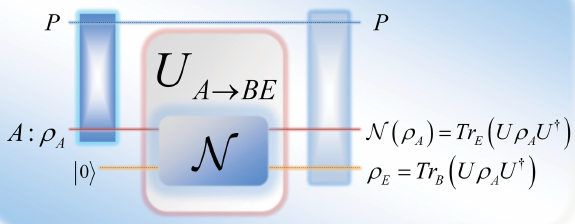
\includegraphics[width=0.6\textwidth]{figures/quantum_communication_quantum_channel.png}
    \caption{Quantum communication through a quantum channel \cite{Gyongyosi_2018}. The channel is represented as the unitary transformation. $P$ refers to the reference system or the purification state. The outputs received by Bob (first) and the environment (second) can be computed using the partial trace operator.}
\end{figure}

We shall see that this definition of quantum capacity satisifies non-negativity, but violates the additivity relation similar to private capacity. We would then examine a special class of quantum channels that satisfies the additive relation for both private and quantum capacity. Moreover, their private and quantum capacities happen to be always equal.

\subsection{Properties of Quantum Capacity}

\begin{theorem}[Non-negativity]
The quantum capacity $Q(\mathcal{N})$ of a quantum channel $\mathcal{N}$ is non-negative.
$$Q(\mathcal{N}) \geq 0$$
\end{theorem}

\begin{proof}
Similar to the non-negativity proofs earlier, we would construct a state that achieves zero coherent information. Since the quantum capacity is the maximum over all such states, it is guaranteed to be non-negative.

Consider the input state $\phi_{AA'}$ to be a product state of the form $\psi_A \otimes \Phi_{A'}$, where the state $A$ is pure. We can evaluate its coherent information as follows.

\begin{align*}
I(A \rangle B)_{\psi \otimes \mathcal{N}(\Phi)} &= S(B)_{\mathcal{N}(\Phi)} - S(AB)_{\psi \otimes \mathcal{N}(\Phi)} \\
&= S(B)_{\mathcal{N}(\Phi)} - S(A)_{\psi} - S(B)_{\mathcal{N}(\Phi)} \\
&= - S(A)_{\psi} \\
&= 0
\end{align*}

The first equality follows from the definition of coherent information. The second makes use of the fact that $AB$ is a product state. The third cancels out common terms, while the fourth makes use of the fact that $A$ is a pure state.
\end{proof}

\begin{theorem}[Non-additivity]
Let $\mathcal{N}_1$ and $\mathcal{N}_2$ represent two quantum channels. The quantum capacity of the combined quantum channel $\mathcal{N}_1 \otimes \mathcal{N}_2$ is not equal to the sum of the individual quantum capacities of $\mathcal{N}_1$ and $\mathcal{N}_2$.
$$Q(\mathcal{N}_1 \otimes \mathcal{N}_2) \neq Q(\mathcal{N}_1) + Q(\mathcal{N}_2)$$
\end{theorem}

\begin{proof}
Consider a private Horodecki channel $\mathcal{N}_H$ and a symmetric channel of unbounded dimension $\mathcal{A}$. These channels are known to have the following properties \cite{Horodecki_1996} \cite{Horodecki_1997} \cite{Smith_2008_Symmetric}.
$$P(\mathcal{N}_H) > 0, Q(\mathcal{N}_H) = 0, Q(\mathcal{A}) = 0$$

Further, we will utilize the following relation between the private capacity and the assisted capacity \cite{Smith_2008}.
$$\frac{1}{2} P(N_H) \leq Q_\mathcal{A}(N_H)$$

Since $P(\mathcal{N}_H) > 0$, it follows that the assisted capacity $Q_\mathcal{A}(\mathcal{N}_H) > 0$. Further, since $\mathcal{A}$ is a symmetric channel of unbounded dimension, the quantum capacity of the joint channel can be related with the assisted capacity as follows \cite{Smith_2008_Symmetric}.
$$Q(\mathcal{N}_H \times \mathcal{A}) = Q_\mathcal{A}(\mathcal{N}_H) > 0$$

Finally, note that $Q(\mathcal{N}_H) + Q(\mathcal{A}) = 0$. We can thus conclude the following relation establishing non-additivity.
$$Q(\mathcal{N}_H \times \mathcal{A}) \neq Q(\mathcal{N}_H) + Q(\mathcal{A})$$
\end{proof}

\begin{theorem}[Relation with other capacities]
The single use capacities of a quantum channel $\mathcal{N}$ are related to each other as:
$$Q(\mathcal{N}) \leq P(\mathcal{N}) \leq C(\mathcal{N})$$
\end{theorem}

\begin{proof}
The reason why $P(\mathcal{N}) \leq C(\mathcal{N})$ holds is easy to see. In both classical and private communication models, our objective is to transmit classical information. Private communication is a specific case of the lesser constrained classical communication through quantum channels. Thus, the classical capacity cannot be lesser than the private capacity.

For proving the other half of the inequality, i.e. $Q(\mathcal{N}) \leq P(\mathcal{N})$, we will consider a pure state that maximizes the quantum capacity. Let $\sigma_{XA'}$ denote the augmented classical-quantum state that correlates with index $x$.

$$\sigma_{XA'} = \sum_{x} p_X(x) \ket{x}\bra{x} \otimes \ket{\phi_x}\bra{\phi_x}_{A'}$$

\begin{align*}
Q(\mathcal{N}) &= \max_{\rho} \left[ S(B)_{\rho} - S(E)_{\rho} \right] \\
&= S(B)_{\sigma} - S(E)_{\sigma} \\
&= S(B)_{\sigma} - S(B|X)_{\sigma} - S(E)_{\sigma} + S(B|X)_{\sigma} \\
&= I(X;B)_{\sigma} - S(E)_{\sigma} + S(E|X)_{\sigma} \\
&= I(X;B)_{\sigma} - I(X;E)_{\sigma} \\
&\leq \max_{\rho} \left[ I(X;B)_{\rho} - I(X;E)_{\rho} \right] \\
&= P(\mathcal{N})
\end{align*}
\end{proof}

The first equality is by definition of quantum capacity. The second equality is by construction of the quantum state. The fourth equality is by the definition of mutual information and by the fact that $\sigma$ on systems $B$ and $E$ is pure when conditioned on $X$. The fifth equality is by the definition of mutual information. The last equality is by the definition of private capacity.

\subsection{Degradable Quantum Channels}

A channel $\mathcal{N}: \mathcal{H}_A \rightarrow \mathcal{H}_B$ can be defined by an isometric embedding $U: \mathcal{H}_A \rightarrow \mathcal{H}_B \otimes \mathcal{H}_E$, followed by a partial trace over the environment system $E$: $\mathcal{N}(\rho) = \mathrm{Tr}_E U(\rho)$. The complementary channel $\mathcal{N}^c: \mathcal{H}_A \rightarrow \mathcal{H}_E$ is defined by: $\mathcal{N}^c(\rho) = \mathrm{Tr}_B U(\rho)$. We regard a quantum channel as degradable if the transmission from the sender end to the environment is noisier than the transmission to the receiver. This is modeled as a result of an additional application of a ``degrading'' channel.

\begin{figure}[H]
    \centering
    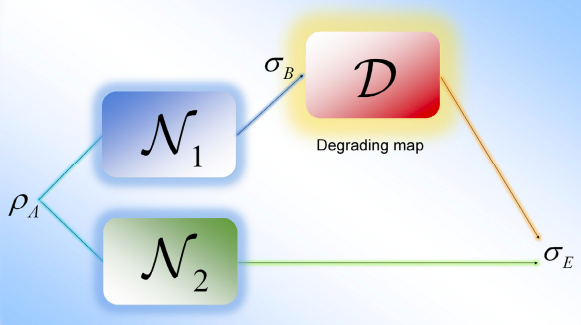
\includegraphics[width=0.6\textwidth]{figures/degradable_quantum_channel.png}
    \caption{The concept of a degradable quantum channel \cite{Gyongyosi2012PropertiesOT}. The environment state can be simulated by the application of the degrading channel on the quantum state received by Bob.}
\end{figure}

\begin{definition}[Degradable Quantum Channel]
A channel $\mathcal{N}: \mathcal{H}_A \rightarrow \mathcal{H}_B$ is called degradable when it may be degraded to its complementary channel $\mathcal{N}^c: \mathcal{H}_A \rightarrow \mathcal{H}_E$, i.e. when there exists a CPTP map $T: \mathcal{H}_B \rightarrow \mathcal{H}_E$ such that
$$\mathcal{N}^c = T \circ \mathcal{N}$$
\end{definition}

\begin{theorem}[Additivity of Quantum Capacity]
Let $\mathcal{N}$ and $\mathcal{M}$ represent two degradable quantum channels. The quantum capacity of the combined quantum channel $\mathcal{N} \otimes \mathcal{M}$ is equal to the sum of the individual quantum capacities of $\mathcal{N}$ and $\mathcal{M}$.
$$Q(\mathcal{N} \otimes \mathcal{M}) = Q(\mathcal{N}) + Q(\mathcal{M})$$
\end{theorem}

\begin{proof}
The reason why $Q(\mathcal{N} \otimes \mathcal{M}) \geq Q(\mathcal{N}) + Q(\mathcal{M})$ holds is easy to see. We can think of a separable input state $\rho_{AB} = \rho_A \otimes \rho_B$ that is maximized indepedently for the two channels. Since the entropy is additive for such states, the joint capacity cannot be lower than the sum of invididual capacities. 

For the reverse direction, consider a pure state $\phi_{AA_1'A_2'}$ as the input to the two channels. Let the following denote the result of the channels, where $\rho_{AB_{1}E_{1}B_{2}E_{2}}$ is a state that maximizes $Q(\mathcal{N} \otimes \mathcal{M})$.
\begin{align*}
\sigma_{AB_{1}E_{1}A_{2}} &= U^{N} \phi (U^{N})^{\dagger} \\
\theta_{AA_{1}B_{1}E_{2}} &= U^{M} \phi (U^{M})^{\dagger} \\
\rho_{AB_{1}E_{1}B_{2}E_{2}} &= (U^{N} \otimes U^{M}) \phi ((U^{N})^{\dagger} \otimes (U^{M})^{\dagger})
\end{align*}

We can write the quantum capacity of the joint channel as follows to show the reverse direction.
\begin{align*}
Q(\mathcal{N} \otimes \mathcal{M}) &= I(A;B_1B_2)_{\rho} \\
&= S(B_1B_2)_{\rho} - S(E_1E_2)_{\rho} \\
&= S(B_1)_{\rho} - S(E_1)_{\rho} + S(B_2)_{\rho} - S(E_2)_{\rho} - [I(B_1;B_2)_{\rho} - I(E_1;E_2)_{\rho}] \\
&\leq S(B_1)_{\rho} - S(E_1)_{\rho} + S(B_2)_{\rho} - S(E_2)_{\rho} \\
&= S(B_1)_{\sigma} - S(AA_2'B_1)_{\sigma} + S(B_2)_{\sigma} - S(AA_1'B_2)_{\sigma} \\
&= I(AA_2';B_1)_{\sigma} + I(AA_1';B_2)_{\sigma} \\
&\leq Q(\mathcal{N}) + Q(\mathcal{M})
\end{align*}

The fourth inequality holds because there is a degrading channel from both $B_1$ to $E_1$ and $B_2$ to $E_2$. This gives us $I(B_1; B_2)_\rho \geq I(E_1; E_2)_\rho$. The fifth inequality holds because the state $\sigma$ on systems $AA_2'B_1E_1$ is pure and the state $\theta$ on systems $AA_1'B_2E_2$ is pure.

Combining the two inequalities establishes the additivity of quantum capacity of degradable channels.
\end{proof}

\begin{theorem}[Additivity of Private Capacity]
Let $\mathcal{N}$ and $\mathcal{M}$ represent two degradable quantum channels. The private capacity of the combined quantum channel $\mathcal{N} \otimes \mathcal{M}$ is equal to the sum of the individual private capacities of $\mathcal{N}$ and $\mathcal{M}$.
$$P(\mathcal{N} \otimes \mathcal{M}) = P(\mathcal{N}) + P(\mathcal{M})$$
\end{theorem}

\begin{proof}
To prove $P(\mathcal{N} \otimes \mathcal{M}) \geq P(\mathcal{N}) + P(\mathcal{M})$, consider the states $\rho$ and $\sigma$ maximizing the private capacity of channels $\mathcal{N}$ and $\mathcal{M}$ respectively. Let $\theta = \rho \otimes \sigma$ be the tensor product of the two states. Then using the additivity of mutual information on tensor product states, we can write the following.
\begin{align*}
P(\mathcal{N}) + P(\mathcal{M}) &= I(X_1;B_1)_{\rho} - I(X_1;E_1)_{\rho} + I(X_2;B_2)_{\sigma} - I(X_2;E_2)_{\sigma} \\
&= I(X_1X_2;B_1B_2)_{\theta} - I(X_1X_2;E_1E_2)_{\theta} \\
&\leq \max_{\alpha} \left[ I(X_1X_2;B_1B_2)_{\alpha} - I(X_1X_2;E_1E_2)_{\alpha} \right] \\
&= P(\mathcal{N} \otimes \mathcal{M})
\end{align*}

To prove the other direction, consider a state $\sigma$ that maximizes $P(\mathcal{N} \otimes \mathcal{M})$ and let $\rho$ be the state that arises from sending $\sigma$ through the joint channel. We can evaluate the quantum capacity of the joint channel as follows.
\begin{align*}
P(\mathcal{N} \otimes \mathcal{M}) &= I(X; B_1B_2)_\sigma - I(X; E_1E_2)_\sigma \\
&= I(XY; B_1B_2)_\sigma - I(XY; E_1E_2)_\sigma - [I(Y; B_1B_2|X)_\sigma - I(Y; E_1E_2|X)_\sigma] \\
&\leq I(XY; B_1B_2)_\sigma - I(XY; E_1E_2)_\sigma \\
&= S(B_1B_2)_\sigma - S(B_1B_2|XY)_\sigma - S(E_1E_2)_\sigma + S(E_1E_2|XY)_\sigma \\
&= S(B_1B_2)_\sigma - S(B_1B_2|XY)_\sigma - S(E_1E_2)_\sigma + S(B_1B_2|XY)_\sigma \\
&= S(B_1B_2)_\sigma - S(E_1E_2)_\sigma \\
&= S(B_1)_\sigma - S(E_1)_\sigma + S(B_2)_\sigma - S(E_2)_\sigma - [I(B_1; B_2)_\sigma - I(E_1; E_2)_\sigma] \\
&\leq S(B_1)_\sigma - S(E_1)_\sigma + S(B_2)_\sigma - S(E_2)_\sigma \\
&\leq \max_\alpha \left[ S(B_1)_\alpha - S(E_1)_\alpha \right] + \max_\beta \left[ S(B_2)_\beta - S(E_2)_\beta \right] \\
&= Q(\mathcal{N}) + Q(\mathcal{M}) \\
&= P(\mathcal{N}) + P(\mathcal{M})
\end{align*}

The second equality holds because of the chain rule for mutual information. The third inequality holds because $I(Y; B_1B_2|X)_\sigma \geq I(Y; E_1E_2|X)_\sigma$ for degradable channels. The fourth inequality uses the definition of mutual information. The fifth inequality uses the fact that state $\sigma$ on systems $B_1B_2E_1E_2$ is pure when conditioning on classical systems $X$ and $Y$. The seventh inequality uses the definition of mutual information. The second last inequality uses the definition of quantum capacity. The last inequality uses the equivalence of private and quantum capacity for degradable channels (proved later).

Combining the two inequalities establishes the additivity of private capacity of degradable channels.
\end{proof}

\begin{theorem}[Equivalence of Private and Quantum Capacity]
For a degradable quantum channel $\mathcal{N}$, the private capacity is equal to the quantum capacity.
$$P(\mathcal{N}) = Q(\mathcal{N})$$
\end{theorem}

\begin{proof}
We will prove $P(\mathcal{N}) \leq Q(\mathcal{N})$ for any degradable channel $\mathcal{N}$. Consider a state $\sigma$ that maximizes the private capacity of the channel $\mathcal{N}$. We can write its private capacity as follows.

\begin{align*}
P(\mathcal{N}) &= I(X;B)_{\sigma} - I(X;E)_{\sigma} \\
&= I(XY;B)_{\sigma} - I(Y;B|X)_{\sigma} - [I(XY;E)_{\sigma} - I(Y;E|X)_{\sigma}] \\
&= I(XY;B)_{\sigma} - I(XY;E)_{\sigma} - [I(Y;B|X)_{\sigma} - I(Y;E|X)_{\sigma}] \\
&\leq I(XY;B)_{\sigma} - I(XY;E)_{\sigma} \\
&= S(B)_{\sigma} - S(B|XY)_{\sigma} - S(E)_{\sigma} + S(E|XY)_{\sigma} \\
&= S(B)_{\sigma} - S(B|XY)_{\sigma} - S(E)_{\sigma} + S(B|XY)_{\sigma} \\
&= S(B)_{\sigma} - S(E)_{\sigma} \\
&\leq \max_\phi \left[ S(B)_{\phi]} - S(E)_{\phi} \right] \\
&= Q(\mathcal{N})
\end{align*}

The second inequality follows from the chain rule of mutual information. The fourth inequality holds because of the property of the degrading channel. The fifth inequality follows from the definition of mutual information. The sixth inequality holds because the state $\sigma$ on
systems $B$ and $E$ is pure when conditioned on classical systems $X$ and $Y$. The last inequality follows from the definiton of quantum capacity of a channel.

Combining this inequality with the inequality proved earlier for all quantum channels, i.e. $Q(\mathcal{N}) \leq P(\mathcal{N}) \leq C(\mathcal{N})$, we can conclude that $P(\mathcal{N}) = Q(\mathcal{N})$ for degradable channels.
\end{proof}


\renewcommand{\pageauthor}{Shreyas Sinha}
\section{Super Additivity of Quantum Channels}

Superadditivity in quantum information theory refers to the phenomenon where
certain types of quantum capacities increase when multiple channels (or multiple
uses of the same channel) are considered, rather than treating each channel
(or use) independently. This property arises because quantum entanglement and
correlations can enhance the effectiveness of the channel when used in a
collective or joint manner. Superadditivity is a fundamental property that
distinguishes quantum information theory from classical information theory.

This Superadditivity is the result of entanglement and other exotic correlation
phenomena that arises in quantum systems. Superadditivity enhances
communication capabilities of quantum channels and allows more communication
than what their classical counterparts could (sometimes even through
zero capacity channels).

\subsection{Classical Capacity}
One manifestation of superadditivity appears in the classical capacity of quantum
channels, particularly through the Holevo information. As we have seen before, the
Holevo Information of a quantum channel is an upper bound on the classical information
that can be transmitted through it. Also as we have seen before, Classical capacity
has been defined in terms of the Holevo information. As a result, it can exhibit
superadditivity when multiple channel uses are considered together. For example, when
encoding information across multiple uses of the channel in an entangled way or by
using complex encoding schemes, the total classical capacity often exceeds what would be
achievable by simply using each channel separately. Thus, superadditivity allows us to
exploit collective encoding and decoding strategies to maximize the amount of classical
information extracted from quantum channels.

Although it is worth noting that we don't yet know the precise mathematics behind why
Holevo information is superadditive, we just know from counter examples that additivity
is not the general case and super additivity can exist.

Mathematically, we write the Holevo information of two channels acting in parallel as:
\begin{equation}
    \chi(\mathcal{N} \otimes \mathcal{M}) \geq \chi(\mathcal{N}) + \chi(\mathcal{M})
\end{equation}
Now, since classical capacity is:
\begin{equation}
    C(\mathcal{N}) = \lim_{n \rightarrow \infty }\frac{1}{n}\chi(\mathcal{N}^{\otimes n})
\end{equation}
For channel $\mathcal{N}\otimes\mathcal{M}$ we have:
\begin{align}\begin{split}
    C(\mathcal{N}\otimes\mathcal{M}) & = \lim_{n \rightarrow \infty }\frac{1}{n}\chi[(\mathcal{N}\otimes\mathcal{M})^{\otimes n}]\\
    & \geq \lim_{n \rightarrow \infty }\frac{1}{n}[\chi(\mathcal{N}^{\otimes n}) + \chi(\mathcal{M}^{\otimes n})]\\
    & = \lim_{n \rightarrow \infty }\frac{1}{n}\chi(\mathcal{N}^{\otimes n}) + \lim_{n \rightarrow \infty }\frac{1}{n}\chi(\mathcal{M}^{\otimes n})\\
    & = C(\mathcal{N} + \mathcal{M})
\end{split}\end{align}

\subsection{Quantum Capacity}
Coherent Information

\subsection{Private Capacity}
\section{Examples of Quantum Channels}

\begin{frame}{Examples of quantum channels - Bit Flip channel}
    We present the \textbf{Bit Flip} channel.\\
    The Bit flip channel, as its name suggests, flips a qubit from $|0\rangle $ to $|1\rangle $ (or $|1\rangle $ to $|0\rangle $) with probability $p$, and
    does nothing with probability $1-p$:
    \begin{equation}
        \mathcal{N}_p(\rho) = (1-p)\rho + pX\rho X = K_0 \rho K_0^\dagger + K_1 \rho K_1^\dagger
    \end{equation}
    Where $X$ is the Pauli X operator:
    \begin{math}
        X = \begin{bmatrix}
            0 & 1\\
            1 & 0
        \end{bmatrix}
    \end{math}\\
    and $K_0 = (\sqrt{1-p})\mathbb{I} $ and $K_1 = (\sqrt{p})X$ are the Kraus operators.\\

    More channel examples will be produced soon along with analyses on the various capacities of these channels.
\end{frame}

\begin{frame}{Example - Erasure channel}
    % \item[Erasure Quantum Channel]{
        The erasure quantum channel $\mathcal{N}_p$ "erases" the input state $\rho$
        with probability $p$ or transmits the state unchanged with probability $(1−p)$
        \begin{equation}
            \mathcal{N}_p(\rho) \rightarrow (1-p)\rho + (p| e \rangle\langle e |)
        \end{equation}
        where $|e\rangle$ is the "erasure state".
        The classical capacity of this channel is given by:
        \begin{equation}
            C(\mathcal{N}_p) = (1-p)\log (d)
        \end{equation}
        Here $d$ is the dimension of the input system. This demonstrates that the channel
        can transmit some classical information only for $0 \leq p < 1$, otherwise the
        classical capacity is $0$.
        
        On the other hand, its quantum capacity is:
        \begin{equation}
            Q(\mathcal{N}_p) = (1-2p)\log (d)
        \end{equation}
        This is similar to classical capacity, except that information can only be transferred
        if $0 \leq p < 1/2$.
    % }
\end{frame}
\begin{frame}{Example - Phase Erasure Channel}
    % \item[Phase Erasure channel] {
        The Phase Erasure channel "erases" (as the name indicates) the phase of its inputs with
        probability $p$ but does not affect the amplitude. The map is expressed as:
        \begin{equation}
            \mathcal{N}(\rho) \rightarrow (1-p)\rho \otimes |0\rangle\langle 0| + p\frac{\rho + Z\rho Z^\dagger}{2}\otimes |1\rangle\langle 1|
        \end{equation}
        The classical capacity of this channel is:
        \begin{equation}
            C(\mathcal{N}) = 1
        \end{equation}
        The quantum capacity of this channel is:
        \begin{equation}
            Q(\mathcal{N}) = (1-p)\log (d)
        \end{equation}
        where the variables hold the same meaning as the last example.
    % }
\end{frame}

\begin{frame}{Superadditivity}
    Graeme Smith and Jon Yard's example:

    A private Horodecki channel and a Symmetric channel may be combined to
    give a quantum channel with non-zero Quantum capacity, even though the
    individual channels have zero quantum capacity individually.
\end{frame}

\renewcommand{\pageauthor}{}
\bibliographystyle{ieeetr}
\bibliography{refs}

\end{document}
